\documentclass{article}
\usepackage{graphicx}
\usepackage[margin=1.5cm]{geometry}
\usepackage{amsmath}

\begin{document}
\twocolumn

\title{Friday warm-up: vectors, displacement, velocity, time, and acceleration}
\author{Prof. Jordan C. Hanson}

\maketitle

\section{Memory Bank}

\begin{enumerate}
\item $\vec{v} = v_x \hat{i} + v_y \hat{j}$ ... Definition of a vector in terms of $\hat{i}$ and $\hat{j}$ components (representing the x-direction and y-direction).
\item $\vec{v} + \vec{w} = (v_x + w_x) \hat{i} + (v_y + w_y) \hat{j}$ ... Vector addition: the $\hat{i}$-components add with each other, and the $\hat{j}$-components add with each other.\
\item $|\vec{v}| = \sqrt{v_x^2 + v_y^2}$ ... The magnitude of the vector
\item $v_x = |\vec{v}| \cos\phi$, $v_y = |\vec{v}| \sin\phi$ ... The x and y-components of the vector, assuming $\phi$ is the angle between $\vec{v}$ and the x-axis.
\item $\Delta \vec{x} = \vec{x}_f - \vec{x}_i$ ... Definition of displacement
\item $\Delta t = t_f - t_i$ ... Definition of time-duration
\item $\vec{v} = \Delta \vec{x}/\Delta t$ ... Definition of velocity
\item $\vec{a} = \Delta \vec{v}/\Delta t$ ... Definition of acceleration
\end{enumerate}

\section{Chapter 2 - Kinematics I}

\begin{enumerate}
\item If $\vec{v} = -3\hat{i} + 3\hat{j}$ km/hr, (a) what is the \textit{magnitude} of $\vec{v}$? (b) Graph $\vec{v}$ in a 2D coordinate system. (c) What is the angle between $\vec{v}$ and the positive x-axis? \\ \vspace{4cm}
\item Suppose a system is moving with the velocity in the previous exercise.  If the system is at the origin of a 2D coordinate system at time $t_i=0$, where will the system be at $t_f = 60$ seconds? \\ \vspace{3cm}
\item Suppose a spacecraft is touching down on the Moon, and it is descending with a constant velocity $\vec{v}_i = -10 \hat{j}$ m s$^{-1}$.  A additional booster is ignited such that, after 10 seconds, the velocity is $\vec{v}_f = -2 \hat{j}$ m s$^{-1}$.  (a) What is the acceleration, $\vec{a}$? (b) Explain why the acceleration should be positive or negative, vertically. \\ \vspace{2cm}
\item A worker is searching for cracks along a stretch of road that is 4 km long (Fig. \ref{fig:1}).  First, he moves +0.5 km in 9 minutes.  Second, he moves -0.5 km in 9 minutes.  Third, he +1 km in 14 minutes.  Finally, he moves -1.75 km in 26 minutes.  (a) What total distance did he travel? (b) What is his \textit{displacement} over 58 minutes? (c) Find the average velocity of the worker.
\end{enumerate}

\begin{figure}
\centering
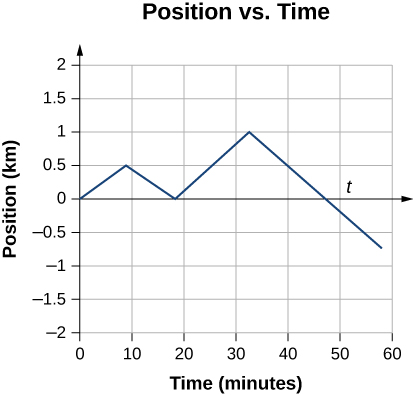
\includegraphics[width=0.45\textwidth]{figures/graph_x_t.jpeg}
\caption{\label{fig:1} A system moves in one dimension with displacement $\vec{x}$ (km) versus time $t$ (min).}
\end{figure}

\end{document}
